\begin{frame}
\frametitle{Participate!}
During the lectures...
\begin{itemize}
\item Don't hesitate to ask questions. Other people in the audience may have
similar questions too.
\item This helps the trainer to detect any explanation that wasn't clear or
detailed enough.
\item Don't hesitate to share your experience, for example to compare Linux
with other operating systems used in your company.
\item Your point of view is most valuable, because it can be similar to your
colleagues' and different from the trainer's.
\item Your participation can make our session more interactive and make the
topics easier to learn.
\end{itemize}
\end{frame}

\begin{frame}
\frametitle{Advise: write down your commands!}
During practical labs, write down all your commands in a text file.
\begin{columns}
\column{0.6\textwidth}
  \begin{itemize}
  \item You can save a lot of time re-using commands in later labs.
  \item This helps to replay your work if you make significant mistakes.
  \item You build a reference to remember commands in the long run.
  \item That's particular useful to keep kernel command line settings
        that you used earlier.
  \item Also useful to get help from the instructor, showing the
        commands that you run.
  \end{itemize}
\code{gedit ~/lab-history.txt}
\column{0.4\textwidth}
  \includegraphics[width=\textwidth]{slides/course-information/text-notes.pdf}
\end{columns}
\end{frame}

\begin{frame}
\frametitle{Cooperate!}
\begin{columns}
\column{0.8\textwidth}
  As in the Free Software and Open Source community,
  cooperation during practical labs is valuable in this training session:
  \begin{itemize}
    \item Use the dedicated Matrix channel for this session
    \item If you complete your labs before other people, don't hesitate to help
          them and investigate the issues they face. The faster we progress as a
          group, the more time we have to explore extra topics.
    \item Explain what you understood to other participants when needed.
          It also helps to consolidate your knowledge.
    \item Don't hesitate to report potential bugs to your instructor.
    \item Don't hesitate to look for solutions on the Internet as well.
    \end{itemize}
\column{0.2\textwidth}
  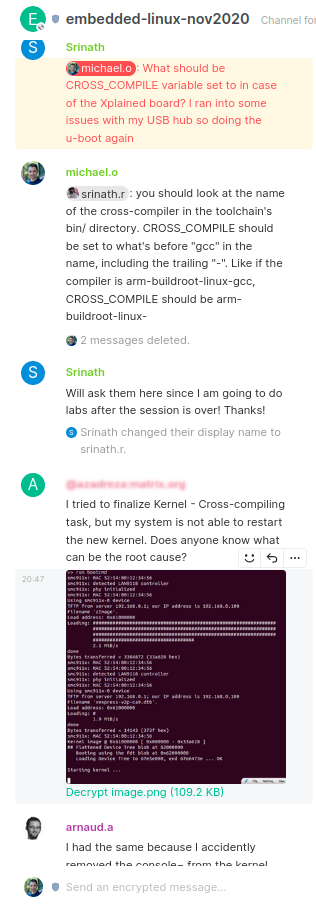
\includegraphics[height=0.8\textheight]{slides/course-information/matrix-screenshot.png}
\end{columns}
\end{frame}
